\section{Directed instruction tests and helper scripts}

\subsection{ISA tests}
Directed tests under \texttt{tests/isa/} exercise every supported instruction
group. Each test writes a deterministic signature to \texttt{0x2000\_0100} and
ships with a golden \texttt{.sig} file. The golden words are generated with the
Spike RISC-V ISA simulator (Section~\ref{sec:spike-golden}).

\subsection{Prerequisites}
The documented workflow assumes:
\begin{itemize}[leftmargin=*]
  \item A bare-metal RISC-V GCC toolchain (e.g. \texttt{riscv64-unknown-elf-gcc} and \texttt{objcopy}).
  \item Python 3 (used for binary-to-hex conversion).
  \item GHDL with VHDL-2008 support (for simulation).
\end{itemize}

On Ubuntu, the documentation suggests installing the basics via APT:
\begin{lstlisting}[style=minrv]
sudo apt update
sudo apt install gcc-riscv64-unknown-elf binutils-riscv64-unknown-elf \
  ghdl python3 python3-pip make
\end{lstlisting}

\paragraph{Optional: Spike (golden signatures)}
\texttt{gen\_golden.sh} and \texttt{check\_goldens.sh} need the Spike ISA
simulator. Spike is not packaged for Ubuntu, so it is built from source:
\begin{lstlisting}[style=minrv]
sudo apt install -y build-essential git device-tree-compiler \
  libboost-regex-dev libboost-system-dev
git clone https://github.com/riscv-software-src/riscv-isa-sim.git
cd riscv-isa-sim && mkdir build && cd build
../configure --prefix=/opt/riscv   # or --prefix=$HOME/.local (no sudo)
make -j"$(nproc)" && sudo make install
export PATH=/opt/riscv/bin:$PATH
spike --help | grep debug-cmd      # check
\end{lstlisting}
Spike is needed only to create or re-check \texttt{.sig} files, not to run the
existing tests.

\paragraph{Optional: schematic generation and DigitalJS interactive simulation}
To generate SVG schematics of RTL entities and to export DigitalJS JSON for
interactive browser-based simulation (see \texttt{scripts/gen\_schematic.sh}):
\begin{lstlisting}[style=minrv]
sudo apt install -y yosys ghdl yosys-plugin-ghdl graphviz
sudo apt install -y nodejs npm
sudo npm install -g netlistsvg
sudo npm install -g yosys2digitaljs
\end{lstlisting}

\subsection{One-test and batch workflows}
The repository provides scripts that build programs (using GCC) and run the
self-checking testbench (GHDL):

\begin{lstlisting}[style=minrv]
./scripts/run_test.sh full_core
./scripts/run_test.sh --trace full_core
./scripts/run_test.sh --fst full_core
./scripts/run_tests.sh
./scripts/run_tests.sh --trace
\end{lstlisting}

Useful environment overrides include \texttt{MAX\_CYCLES} (for longer programs),
\texttt{FORWARDING\_ENABLE=false} (stall-only hazards), and tool-path variables
such as \texttt{RISCV\_GCC} and \texttt{RISCV\_OBJCOPY}. For simulation, the
scripts also honor \texttt{GHDL} and \texttt{GHDL\_STD} and provide a
\texttt{--verbose}/\texttt{VERBOSE=1} mode to echo the underlying GHDL commands.
To keep the repository root clean (and to avoid collisions when running multiple
tests in parallel), the scripts isolate GHDL work libraries and elaboration
executables under \texttt{build/ghdl/} by default (override with
\texttt{GHDL\_WORKDIR}).

\subsection{Waveform dumps (GTKWave)}
For waveform-first debugging, the scripts can dump waveforms directly from GHDL:
\begin{itemize}[leftmargin=*]
  \item \texttt{--fst}: fast, compact waveform format (recommended).
  \item \texttt{--vcd}: widely supported text waveform.
  \item \texttt{--wave}: GHDL's \texttt{.ghw} format.
\end{itemize}

\begin{lstlisting}[style=minrv]
./scripts/run_test.sh --fst addi_only
./scripts/view_wave.sh build/waves/addi_only.fst
\end{lstlisting}

\subsection{Unit-level testbenches}
For component bring-up without building a program image, run unit testbenches:
\begin{lstlisting}[style=minrv]
./scripts/run_unit_tb.sh regfile
./scripts/run_unit_tb.sh --fst alu
\end{lstlisting}

\subsection{DigitalJS interactive simulation}
\label{sec:digitaljs}
\texttt{gen\_schematic.sh --digitaljs} exports a DigitalJS-compatible JSON that you
can upload to \url{https://digitaljs.tilk.eu/}.  DigitalJS is both a schematic
viewer \emph{and} an interactive simulator: you drive inputs by clicking and watch
values propagate through the gates.  It acts as a visual complement to GTKWave
(for leaf modules) and to the GHDL full-core tests (for the whole pipeline).  It
is not a replacement for the signature-checked \texttt{run\_test.sh} /
\texttt{run\_tests.sh} flows -- those remain the authoritative pass/fail.

\paragraph{Automatic clock and reset ergonomics}
The \texttt{--digitaljs} post-processor calls \texttt{yosys2digitaljs}'s
\texttt{io\_ui()} helper, which remaps raw port devices into simulator-UI
widgets so the exported circuit is immediately runnable without manual clock
toggling: a 1-bit \texttt{Input} named \texttt{clk} becomes a
self-ticking \texttt{Clock} device, any other 1-bit \texttt{Input} (e.g.
\texttt{reset}) becomes a one-click \texttt{Button}, multi-bit \texttt{Input}s
become \texttt{NumEntry} typeable fields, and outputs become \texttt{Lamp} /
\texttt{NumDisplay}.  Upload, press the simulator's run button (auto-pressed by default when loading the .json file), and click
\texttt{reset} once and then click again to create a reset pulse -- the clock runs on its own.

\paragraph{Simple modules (leaf entities)}
Export a single entity and open it in DigitalJS:
\begin{lstlisting}[style=minrv]
./scripts/gen_schematic.sh --digitaljs alu
./scripts/gen_schematic.sh --digitaljs regfile
./scripts/gen_schematic.sh --digitaljs extend
\end{lstlisting}
Upload \texttt{build/schematics/<entity>.digitaljs.json} and toggle inputs.

\paragraph{Full pipeline with real firmware (\texttt{--mem-init})}
Yosys synthesis excludes the \texttt{synthesis translate\_off} guards in
\texttt{mem\_init\_pkg.vhd}, so every memory cell in the exported netlist has
an all-zero initial state.  The \texttt{--mem-init} flag patches the
\texttt{\$mem}/\texttt{\$mem\_v2} INIT parameter with the real hex images
before \texttt{yosys2digitaljs} converts the netlist, giving the DigitalJS
interactive simulation a faithful firmware image:
\begin{lstlisting}[style=minrv]
./scripts/build_prog.sh tests/isa/full_core.c full_core
./scripts/gen_schematic.sh --digitaljs \
    --mem-init imem_dp=build/full_core.text.hex \
    --mem-init dmem=build/full_core.data.hex \
    top
\end{lstlisting}
Upload the resulting \texttt{build/schematics/top.digitaljs.json} to
\url{https://digitaljs.tilk.eu/} to step through the pipeline with the program
already loaded in memory (Figure~\ref{fig:digitaljs-top}).  The
\texttt{--mem-init} injection only works on the
hierarchical (default) netlist where \texttt{imem\_dp} and \texttt{dmem} are
distinct modules; under \texttt{--flat} the modules merge into the top level
and the injection becomes a no-op (a warning is printed).

\begin{figure}[ht]
  \centering
  \fbox{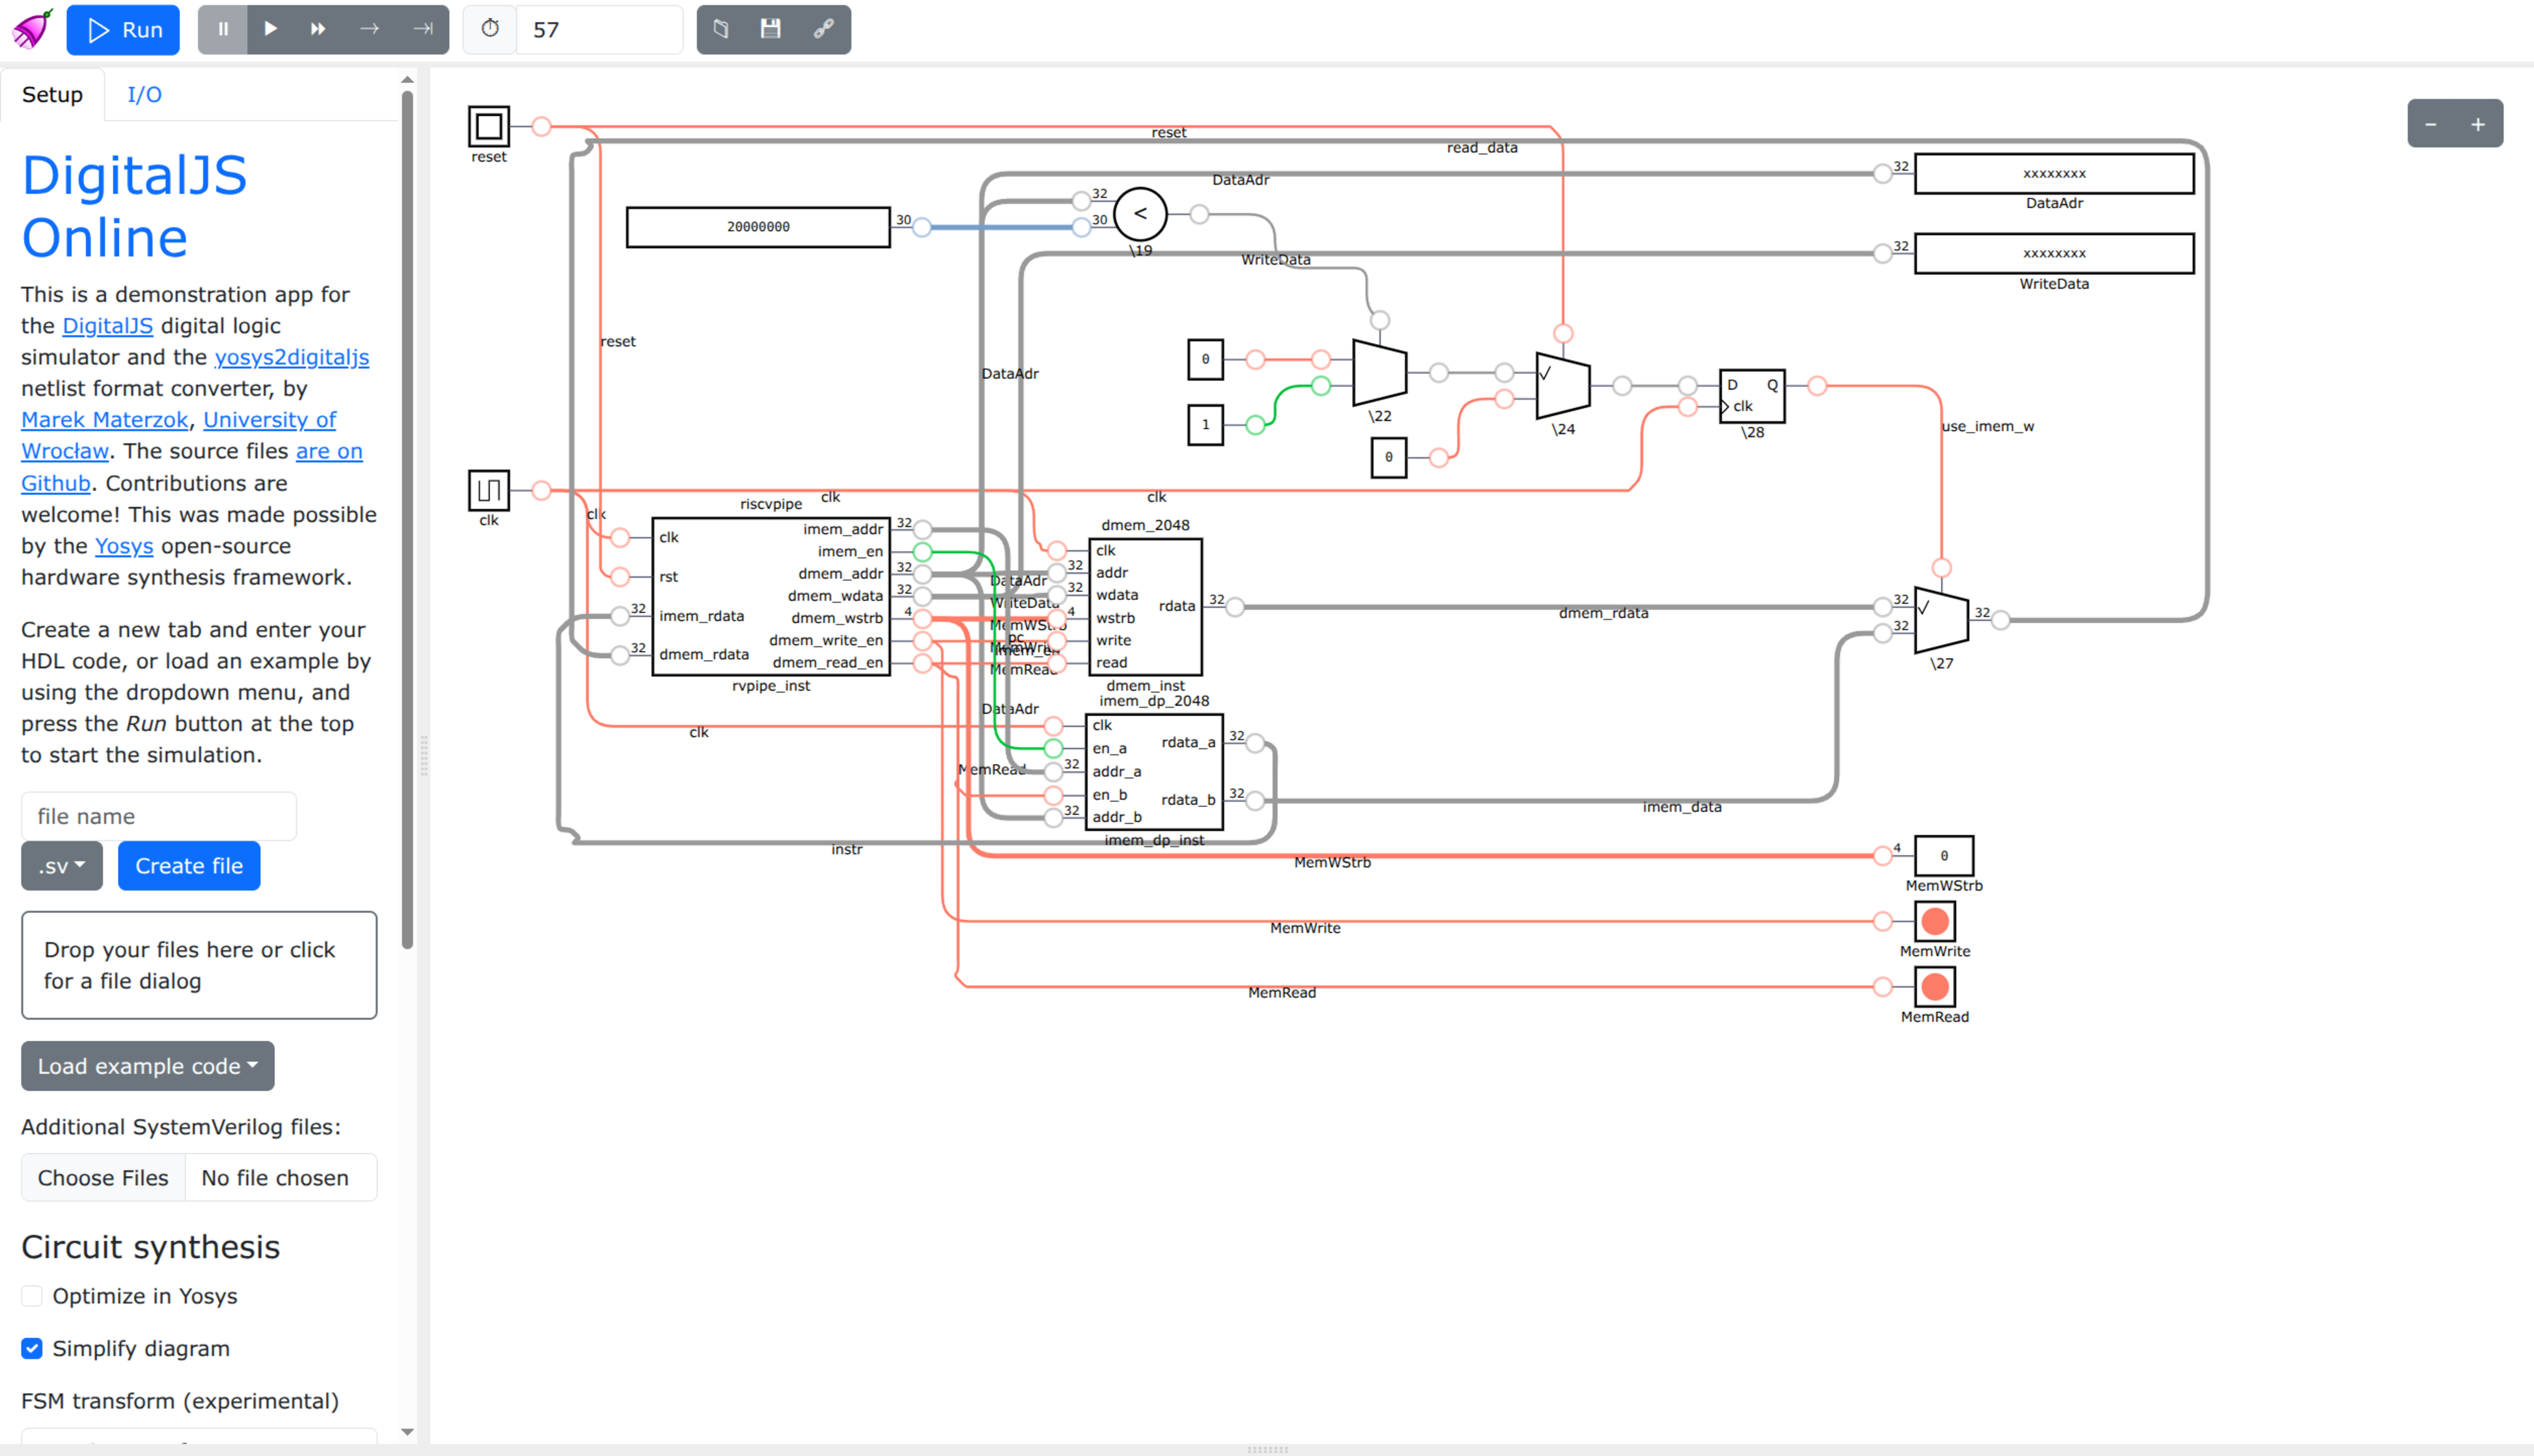
\includegraphics[scale=0.18]{digitaljs-top.pdf}}
  \caption{DigitalJS simulation of the full\_core.c program running on MinRV32.}
  \label{fig:digitaljs-top}
\end{figure}

\subsection{Trace output (optional)}
Both the GHDL-driven scripts and the Vivado documentation describe an optional
per-instruction trace that prints decoded assembly and key control selections
grouped by stage. This is designed as a teaching aid: it links what the program
is doing (assembly) to what the controller and hazard logic are doing (mux and
enable choices).

When the hazard unit takes action (stall/flush/forward), the trace prints an
additional \texttt{HAZARD:} line showing stall/flush decisions plus the
forwarding-source selects for the E-stage operands:
\begin{lstlisting}[style=minrv]
HAZARD: StallF=stall StallD=stall FlushD=keep FlushE=flush FwdA=rf FwdB=rf
\end{lstlisting}
\noindent
\texttt{FwdA/FwdB} select \texttt{rf} (regfile), \texttt{M} (Memory stage), or
\texttt{W} (Writeback stage). The hazard line is only printed when something is
asserted or forwarded.

\subsection{Authoring new tests}
New tests can be written as assembly (\texttt{.S}) or freestanding C
(\texttt{.c}) under \texttt{tests/isa/}. The expected flow is:
\begin{enumerate}[leftmargin=*]
  \item Write a deterministic workload using only the supported instruction subset.
  \item Write final observation words into the signature buffer at \texttt{0x2000\_0100}.
  \item Generate the golden signature with Spike:
  \texttt{./scripts/gen\_golden.sh --words N --write <name>} runs the same
  program on the Spike reference model, reads \texttt{N} words from the signature
  window at \texttt{0x2000\_0100}, and writes \texttt{tests/isa/<name>.sig}
  (Section~\ref{sec:spike-golden}). Do not store raw code or \texttt{.rodata}
  addresses in the signature (Section~\ref{sec:spike-addr}). (Compiling the C for
  the host x86 architecture is \emph{not} a reliable oracle, since 32-bit
  overflow and shift semantics may differ from RV32I.)
  \item Re-run via \texttt{scripts/run\_test.sh <name>} for regression.
\end{enumerate}

\subsection{Golden signatures with Spike}
\label{sec:spike-golden}
The expected \texttt{.sig} words come from Spike, the RISC-V reference ISA
simulator. Spike does not depend on the RTL, so it is an independent oracle for
the design under test.
\begin{lstlisting}[style=minrv]
./scripts/gen_golden.sh factorial                 # print, save build/golden/factorial.sig
./scripts/gen_golden.sh --check factorial         # compare with tests/isa/factorial.sig
./scripts/gen_golden.sh --words 4 --write my_test # create tests/isa/my_test.sig
./scripts/check_goldens.sh                        # check every tests/isa/*.sig
\end{lstlisting}
\texttt{gen\_golden.sh} builds the test with \texttt{build\_prog.sh} (same
compiler flags as the core) and the linker script \texttt{link\_spike.ld}. It
runs the ELF on Spike in debug mode for \texttt{SPIKE\_MAX\_INSNS} instructions
(default 1\,000\,000) and checks that the PC is parked in the final self-loop.
It then reads the signature window and writes \texttt{build/golden/<name>.sig},
one lowercase hex word per line. The word count is \texttt{--words N} or the
line count of the existing \texttt{.sig} file. \texttt{--write} copies the result
to \texttt{tests/isa/<name>.sig}, and \texttt{--check} compares it with that
file. \texttt{check\_goldens.sh} runs \texttt{--check} for every test. The
environment variables \texttt{SPIKE}, \texttt{SPIKE\_ISA} (default
\texttt{rv32i}), and \texttt{SPIKE\_MAX\_INSNS} select the binary, the ISA
string, and the instruction budget.

\paragraph{Spike vs MinRV32 code addresses}
\label{sec:spike-addr}
Spike reserves the low address space for its debug module
(\texttt{0x0000\_0000}--\texttt{0x0000\_0FFF}) and boot ROM (from
\texttt{0x1000}), so instruction memory cannot sit at \texttt{0x0} as it does on
MinRV32. \texttt{link\_spike.ld} moves the code to \texttt{0x8000\_0000};
data memory does not move.

\begin{center}
\begin{tabularx}{\linewidth}{@{}X l l@{}}
\toprule
Item & MinRV32 (\texttt{link.ld}) & Spike (\texttt{link\_spike.ld}) \\
\midrule
\texttt{.init}, \texttt{.text}, \texttt{.rodata} & \texttt{0x0000\_0000} & \texttt{0x8000\_0000} \\
\texttt{.data}, \texttt{.bss}, stack top & \texttt{0x2000\_0000}\ldots{} / \texttt{0x2000\_2000} & same \\
signature window & \texttt{0x2000\_0100} & same \\
\bottomrule
\end{tabularx}
\end{center}

Stores to the signature window go to the same address on both, so only the
stored \emph{value} can differ. A golden word is affected when the value is, or is
computed from, the address of code or \texttt{.rodata}; under Spike it is larger
by \texttt{0x8000\_0000}. Affected values include:
\begin{itemize}[leftmargin=*]
  \item function pointers (\texttt{(uint32\_t)\&main});
  \item label addresses (\texttt{la t0, label} followed by a store of \texttt{t0});
  \item addresses of string literals or \texttt{const} tables;
  \item raw \texttt{jal}/\texttt{jalr} link values and raw \texttt{auipc} results.
\end{itemize}
Unaffected values are arithmetic and logic results, values loaded \emph{from}
\texttt{.rodata} (as in \texttt{lui\_auipc.S}), data-memory addresses, and
differences between two code addresses (as in \texttt{branch\_jump.S}). To use a
code address in a test, store an offset such as
\texttt{(uint32\_t)\&f - (uint32\_t)\&\_start}, which is the same under both
links. A program that stores \texttt{(uint32\_t)\_start + 4} and
\texttt{(uint32\_t)\&main - (uint32\_t)\_start} gives
\texttt{00000004 00000010} on the core and \texttt{80000004 00000010} on Spike.
A \texttt{--check} mismatch of exactly \texttt{0x8000\_0000} means that a code
address has leaked into the signature. Moving the core's code to
\texttt{0x8000\_0000} would remove this difference
(Section~\ref{sec:future-memmap}).

\paragraph{Other Spike vs MinRV32 differences}
\label{sec:spike-other}
In the cases below, the two simulators run the same program differently, so a
golden word can differ even though both run the same code. None of the current tests hits
them.

\emph{Register values at \texttt{\_start}.} Spike starts in its boot ROM, which
leaves \texttt{t0} = \texttt{0x8000\_0000} (the entry address), \texttt{a1} =
\texttt{0x0000\_1020} (the device-tree address), and \texttt{a0} = \texttt{0}
(\texttt{mhartid}). On the core every register is \texttt{0} after reset. Write
every register before you read it; do not rely on reset values.

\emph{Cases the core does not trap but Spike does.} The core has no
exceptions. Spike raises one in the cases below. Because \texttt{mtvec} is
\texttt{0}, Spike then stays at PC \texttt{0x0000\_0000}.
\begin{center}
\begin{tabularx}{\linewidth}{@{}l X l@{}}
\toprule
Case & MinRV32 & Spike \\
\midrule
Misaligned load/store & Ignores the low address bits (a word uses the aligned
word, a halfword uses address bit~1): \texttt{lw} from \texttt{0x2000\_0109}
reads \texttt{0x2000\_0108}. & Misaligned exception \\
Outside the memory windows & Wraps the address into the 8\,KiB array
(\texttt{0x2000\_2000} reads \texttt{0x2000\_0000}). Loads below
\texttt{0x2000\_0000} read IMEM; stores always write DMEM. & Access fault \\
\texttt{ecall}, \texttt{ebreak}, undecoded & No-op & Exception \\
\bottomrule
\end{tabularx}
\end{center}
CSR instructions do not assemble with \texttt{-march=rv32i}, so they cannot
reach either simulator. \texttt{gen\_golden.sh} does not detect a trap: the
trap loop at PC \texttt{0x0} looks like the final self-loop, so the script
reads whatever the signature window holds at that point, often zeros. In
\texttt{build/golden/<name>.spike.log} the two PC values are an address in
\texttt{0x8000\_xxxx} after a normal run and \texttt{0x00000000} after a trap.

\subsection{Running a program on Spike by hand}
\label{sec:spike-manual}
Spike does not compile anything. It is an instruction-set simulator: it loads an
ELF file of RISC-V machine code and executes it one instruction at a time. A C or
assembly source is first compiled and linked by the RISC-V GCC toolchain, and the
resulting ELF is then run on Spike. \texttt{gen\_golden.sh} does these steps
automatically; by hand, from the repository root:
\begin{lstlisting}[style=minrv]
# 1. Compile and link for Spike (code at 0x8000_0000); .c or .S
LINKER_SCRIPT=$PWD/link_spike.ld ./scripts/build_prog.sh \
    tests/isa/factorial.c factorial.spike
# 2. Machine code and symbol addresses
riscv64-unknown-elf-objdump -d build/factorial.spike.elf | less
riscv64-unknown-elf-nm build/factorial.spike.elf   # 80000068 T main
# 3. Start Spike in its interactive debugger
spike -d --isa=rv32i -m0x80000000:0x2000,0x20000000:0x2000 \
    build/factorial.spike.elf
\end{lstlisting}
\texttt{-d} starts the interactive debugger, halted before the first
instruction. \texttt{--isa=rv32i} selects the base ISA of the core.
\texttt{-m...} creates two 8\,KiB memories, code at \texttt{0x8000\_0000} and
data at \texttt{0x2000\_0000} (the MinRV32 DMEM, so the signature window is at
\texttt{0x2000\_0100}). The warning \texttt{tohost and fromhost symbols not in
ELF} is expected: the tests are freestanding, have no \texttt{printf}, and report
their results in the signature window. The tests never exit (they end in a
self-loop), so without \texttt{-d} Spike runs until Ctrl+C. The same commands can
be run in batch with \texttt{--debug-cmd=<file>}, which is how
\texttt{gen\_golden.sh} works (its file is
\texttt{build/golden/<name>.spike.cmd}).

\subsection{Stepping through a program in Spike's debugger}
\label{sec:spike-debug}
Spike shows a \texttt{:} prompt. Execution begins in the boot ROM at
\texttt{0x1000}, which runs five instructions and jumps to \texttt{\_start} at
\texttt{0x8000\_0000}. Most commands take a core number, always \texttt{0} here;
\texttt{help} lists all of them.

\begin{center}
\small
\begin{tabularx}{\linewidth}{@{}l X@{}}
\toprule
Command & Effect \\
\midrule
Enter & run one instruction and print it (\texttt{run 1}) \\
\texttt{run N} / \texttt{r N} & run \texttt{N} instructions, printing each one \\
\texttt{rs N} & run \texttt{N} instructions silently \\
\texttt{run} & run until Ctrl+C, which returns to the prompt \\
\texttt{pc 0}, \texttt{insn 0} & show the PC, or the instruction at the PC \\
\texttt{reg 0}, \texttt{reg 0 a0} & show all registers, or one (ABI names work) \\
\texttt{mem 0x20000100} & show memory at a physical address (signature word 0) \\
\texttt{until pc 0 0x80000068} & run until the PC reaches an address (here \texttt{main}) \\
\texttt{untiln pc 0 <addr>} & the same, printing each instruction \\
\texttt{until reg 0 a0 0x2d0} & run until a register holds a value \\
\texttt{until mem 0x20000100 0x2d0} & run until a memory word holds a value \\
\texttt{q} & quit \\
\bottomrule
\end{tabularx}
\end{center}

A short session with \texttt{factorial.c} (Spike output after each command):
\begin{lstlisting}[style=minrv]
: pc 0
0x00001000                              # in the boot ROM
: r 3
core   0: 0x00001000 (0x00000297) auipc   t0, 0x0
core   0: 0x00001004 (0x02028593) addi    a1, t0, 32
core   0: 0x00001008 (0xf1402573) csrr    a0, mhartid
: until pc 0 0x80000068                 # run to main
: insn 0
0xff010113 addi    sp, sp, -16
: reg 0 sp
0x20002000                              # stack top (__stack_top)
: reg 0 ra
0x8000000c                              # return address: self-loop in _start
: r 2
core   0: 0x80000068 (0xff010113) addi    sp, sp, -16
core   0: 0x8000006c (0x00600513) li      a0, 6
: until mem 0x20000100 0x2d0            # until sig[0] = 6! is stored
: pc 0
0x80000080                              # the instruction after the store
: mem 0x20000100
0x000002d0                              # the value in factorial.sig
: q
\end{lstlisting}
The PCs printed by Spike are \texttt{0x8000\_0000} higher than on the core
because of the Spike link (Section~\ref{sec:spike-addr}); the instructions and
the data values are the same. \texttt{./scripts/run\_test.sh --trace factorial}
shows the same instructions on the core as they pass through the five pipeline
stages.

\subsection{Script roles (high level)}
\begin{itemize}[leftmargin=*]
  \item \texttt{build\_prog.sh}: compile and emit \texttt{.text.hex}/\texttt{.data.hex} under \texttt{build/} (and print a size summary for IMEM/DMEM).
  \item \texttt{run\_test.sh}: build one test, run the VHDL testbench, compare signatures, stop on first mismatch.
  \item \texttt{gen\_golden.sh}: run one test on Spike and produce its golden signature (\texttt{--write} to update \texttt{tests/isa/<name>.sig}, \texttt{--check} to compare with it).
  \item \texttt{check\_goldens.sh}: run \texttt{gen\_golden.sh --check} for every test with a \texttt{.sig} file (match/differ summary).
  \item \texttt{run\_tests.sh}: iterate over all tests with \texttt{.sig} files for regression runs (optional \texttt{--trace} / \texttt{--verbose}).
  \item \texttt{clean.sh}: remove build and simulator artifacts (\texttt{build/}, \texttt{tmp/} if present, and any \texttt{work-obj*.cf}/\texttt{e\string~*} leftovers).
  \item \texttt{bin\_to\_hex.py}: convert raw little-endian binaries into newline-delimited 32-bit hex words (advanced: \texttt{--word-bytes}).
  \item \texttt{run\_unit\_tb.sh}: build and run a single unit-level testbench from \texttt{sim/unit/} (e.g.\ \texttt{alu}, \texttt{regfile}). Accepts \texttt{--fst}/\texttt{--vcd}/\texttt{--wave} for waveform dumps.
  \item \texttt{run\_unit\_tests.sh}: batch driver that iterates over every \texttt{sim/unit/tb\_*.vhd} testbench and calls \texttt{run\_unit\_tb.sh} for each one (pass/fail summary at the end).
  \item \texttt{view\_wave.sh}: convenience wrapper that opens a waveform file in GTKWave (if installed).
  \item \texttt{gen\_schematic.sh}: generate SVG schematics of RTL modules via Yosys (GHDL plugin) + netlistsvg. Supports depth-limited flattening (\texttt{--flat N}), selective sub-module expansion (\texttt{--expand <entity>}), and memory initialisation for DigitalJS simulation (\texttt{--mem-init <module>=<hex>}). Requires extra packages; see above.
  \item \texttt{mem\_init\_inject.py}: patch a Yosys JSON netlist by writing hex-file contents into the \texttt{INIT} parameter of \texttt{\$mem}/\texttt{\$mem\_v2} cells. Called automatically by \texttt{gen\_schematic.sh --mem-init}; can also be used standalone.
  \item \texttt{vhdl\_sources.sh}: shared helper sourced by the simulation scripts to provide ordered VHDL compile lists (\texttt{VHDL\_RTL\_SOURCES}, \texttt{VHDL\_SIM\_SOURCES}). Not executed directly.
\end{itemize}
